\section{Interpretation of the Contract Variance Factor}\label{sec:supp_sigma_decomp}

The scenario model assigned a variance state to each contract rather than one instantaneous variance state to the underlying. The following continuous-time process motivated the Euler update for a fixed target:
\begin{equation}\label{eq:level_sde}
    dv_{a,t}=\kappa(\bar v_{a,t}-v_{a,t})\,dt
    +\sigma_v\sqrt{v_{a,t}}\,dW_{a,t}.
\end{equation}
Contract $a$ indexes ticker, strike, and expiration. The target $\bar v_{a,t}$ in~\eqref{eq:theta} changes with current moneyness and calendar DTE. If that target were held fixed and a stationary distribution existed, its mean would equal $\bar v_a$. In the implemented scenario, however, the target moved at every trading date and the hard floor in~\eqref{eq:euler} altered the unconstrained square-root process. We therefore use the stationary result only as motivation for mean reversion, not as a claim about the simulated distribution. At entry, $v_{a,0}=\bar v_{a,0}$ reproduces the fitted IV product exactly. Thereafter, $\sigma_{a,t}^2=v_{a,t}$ supplies the lattice input. The fitted level and neural shape are not separately identified: shifting a constant between $\ln\theta_i$ and the network output bias leaves $\theta_i\psi_i$ unchanged. This does not change fitted IV or scenario output, but it prevents separate economic interpretation of the two components.

\section{Calibration Details}\label{sec:supp_sector_nn}

The snapshot labels, capture timestamps, and underlying-session dates did not always coincide. Table~\ref{tab:corpus_dates} preserves these fields for the frozen corpus described in the main Results. All dates are in 2026. The May 11 underlying-session snapshot was captured on May 12. Temporal earnings splits followed snapshot-directory labels, and the May 11 holdout followed the underlying-session date. The first snapshot contained 23 tickers and the remaining snapshots contained 31. The \href{https://github.com/varnerlab/heston_implied_volatility_model}{source repository} provides experiment drivers and reproduction instructions. Its frozen corpus manifest records each file's SHA-256 hash and filtered row count. Saved ablation outputs also include pilot constants, path-level marks, numerical audits, and copies of the computational sources so that the reported comparisons can be traced to their inputs.
\begin{table}[H]
\centering
\caption{Frozen corpus provenance. Temporal earnings splits used snapshot labels; the May 11 single-date holdout used the underlying-session field. The first snapshot label is April 14 although its underlying close was from April 13.}\label{tab:corpus_dates}
\begin{tabular}{lllr}
\toprule
Snapshot label & Capture date & Underlying session & Rows \\
\midrule
04-14-2026 & 2026-04-14 & 2026-04-13 & 18,250 \\
04-15-2026 & 2026-04-15 & 2026-04-15 & 17,711 \\
04-16-2026 & 2026-04-16 & 2026-04-16 & 18,344 \\
04-17-2026 & 2026-04-17 & 2026-04-17 & 17,281 \\
04-21-2026 & 2026-04-21 & 2026-04-21 & 16,760 \\
04-22-2026 & 2026-04-22 & 2026-04-22 & 15,551 \\
04-23-2026 & 2026-04-24 & 2026-04-23 & 11,482 \\
04-24-2026 & 2026-04-24 & 2026-04-24 & 15,351 \\
04-27-2026 & 2026-04-27 & 2026-04-27 & 11,379 \\
04-28-2026 & 2026-04-28 & 2026-04-28 & 16,776 \\
04-29-2026 & 2026-04-30 & 2026-04-30 & 16,811 \\
05-01-2026 & 2026-05-04 & 2026-05-01 & 14,825 \\
05-06-2026 & 2026-05-07 & 2026-05-06 & 17,293 \\
05-08-2026 & 2026-05-08 & 2026-05-08 & 12,293 \\
05-11-2026 & 2026-05-12 & 2026-05-11 & 14,442 \\
\bottomrule
\end{tabular}

\end{table}
\FloatBarrier

\begin{table}[H]
\centering
\caption{Sector partition of the 31-ticker ladder across fifteen snapshots. Counts are filtered observations used in calibration.}\label{tab:sector_map}
\resizebox{\textwidth}{!}{%
\begin{tabular}{lrl}
\toprule
Sector & Observations & Tickers \\
\midrule
ETF        & 102{,}738 & IWM, QQQ, SPY \\
Technology &  68{,}334 & AAPL, AMD, AVGO, GOOG, INTC, META, MSFT, MU, NVDA, QCOM \\
Healthcare &  26{,}387 & ABBV, AMGN, BMY, JNJ, LLY, MRNA, PFE, UNH \\
Financials &  17{,}938 & BAC, GS, JPM, WFC \\
Retail     &  11{,}320 & TGT, UPS, WMT \\
Energy     &   7{,}832 & CVX, OXY, XOM \\
\bottomrule
\end{tabular}}
\end{table}

\begin{table}[H]
\centering
\caption{In-sample RMSE by sector, in volatility percentage points. The sector network improved on the global neural network in every group, while technology and healthcare retained the largest errors.}\label{tab:per_sector}
\begin{tabular}{lrrrr}
\toprule
Sector & Parametric & Global NN & Sector NN & Observations \\
\midrule
ETF        & 10.54 &  8.69 &  6.10 & 102{,}738 \\
Financials &  9.05 &  7.79 &  6.70 &  17{,}938 \\
Energy     &  9.36 &  8.24 &  7.88 &   7{,}832 \\
Retail     & 11.73 & 10.23 &  9.50 &  11{,}320 \\
Healthcare & 13.49 & 12.71 & 12.53 &  26{,}387 \\
Technology & 15.58 & 15.31 & 14.47 &  68{,}334 \\
\bottomrule
\end{tabular}
\end{table}

\begin{table}[H]
\centering
\caption{Largest per-ticker in-sample RMSE reductions among the 29 qualified tickers. In total, 21 qualified tickers improved and eight worsened; the combined per-ticker-plus-fallback model reduced pooled RMSE from 10.24 to 9.73 volatility percentage points. The BMY and PFE fits retained their sector surfaces.}\label{tab:per_ticker_comparison}
\begin{tabular}{lrrrr}
\toprule
Ticker & Observations & Sector NN & Per-ticker NN & Reduction \\
\midrule
JNJ  & 2{,}190 & 11.14 &  7.17 & 3.97 \\
MRNA & 2{,}851 & 17.49 & 13.74 & 3.76 \\
AAPL & 6{,}594 & 14.30 & 12.59 & 1.70 \\
INTC & 3{,}417 & 17.78 & 16.29 & 1.49 \\
AMGN & 3{,}383 & 13.36 & 12.14 & 1.21 \\
MU   & 6{,}619 & 18.45 & 17.26 & 1.19 \\
NVDA & 5{,}805 & 10.14 &  9.15 & 0.99 \\
\bottomrule
\end{tabular}
\end{table}

\begin{table}[H]
\centering
\caption{Mean IV near the money in the May 11 smile panels (Fig.~\ref{fig:per_ticker_panels}). Each row uses the plotted calls and puts with $0.98\le K/S\le1.02$ at the indicated calendar days to expiry (DTE). Observed and predicted IV are percentages; bias is mean per-ticker predicted IV minus observed IV in percentage points. Predictions use the saved fifteen-date fit evaluated at each observed contract. The NVDA subset contains only two observations.}\label{tab:smile_date_bias}
\begin{tabular}{lrrrrr}
\toprule
Ticker & DTE & $N$ & Observed IV & Predicted IV & Bias \\
\midrule
SPY & 7 & 52 & 13.57 & 13.75 & +0.18 \\
NVDA & 7 & 2 & 38.65 & 34.02 & -4.62 \\
MSFT & 9 & 14 & 28.47 & 37.92 & +9.45 \\
LLY & 11 & 20 & 38.59 & 46.49 & +7.90 \\
GS & 11 & 24 & 32.06 & 31.74 & -0.32 \\
AVGO & 9 & 14 & 49.08 & 43.72 & -5.37 \\
\bottomrule\end{tabular}

\end{table}

\begin{table}[H]
\centering
\caption{May 11 price-error summary for the contracts plotted in Fig.~\ref{fig:price_error}. Dollar errors are absolute differences from the market mid. The per-ticker column used a per-ticker surface where qualified and a sector fallback otherwise; the market-IV reference passed each contract's reported IV to the same 200-step CRR lattice.}\label{tab:price_error_summary}
\begin{tabular}{lrrrrrr}
\toprule
Ticker & DTE & $N$ & Half-spread & Per-ticker error & Inside spread & Market-IV error \\
\midrule
SPY  &  7 & 176 & \$0.03 & \$0.12 & 33\% & \$0.01 \\
NVDA &  7 &  34 & \$0.04 & \$0.13 & 35\% & \$0.12 \\
LLY  & 11 & 156 & \$2.98 & \$4.01 & 30\% & \$0.67 \\
GS   & 11 & 145 & \$1.56 & \$0.46 & 88\% & \$0.12 \\
\bottomrule
\end{tabular}
\end{table}

\begin{table}[H]
\centering
\caption{Best and worst ticker-level in-sample RMSE under the sector networks. Errors are in volatility percentage points.}\label{tab:worst_tickers}
\begin{tabular}{llrrl}
\toprule
Rank & Ticker & Observations & RMSE & Sector \\
\midrule
\multicolumn{5}{l}{\emph{Best five}} \\
 1 & GS   &  8{,}772 & 5.40 & Financials \\
 2 & SPY  & 42{,}224 & 6.02 & ETF \\
 3 & IWM  & 21{,}368 & 6.11 & ETF \\
 4 & QQQ  & 39{,}146 & 6.17 & ETF \\
 5 & JPM  &  3{,}720 & 6.18 & Financials \\
\midrule
\multicolumn{5}{l}{\emph{Worst five}} \\
27 & PFE  &  1{,}300 & 17.66 & Healthcare \\
28 & AMD  &  4{,}566 & 17.74 & Technology \\
29 & INTC &  3{,}417 & 17.78 & Technology \\
30 & MU   &  6{,}619 & 18.45 & Technology \\
31 & QCOM &  3{,}375 & 21.46 & Technology \\
\bottomrule
\end{tabular}
\end{table}

\FloatBarrier
\subsection{Single-date holdout}\label{sec:supp_loo}

We held out May 11, 2026, to examine whether the sector surfaces transferred to a nearby date within the observed period. We retrained on the other fourteen dates and calculated input-standardization constants from those training rows alone. Pooled test error exceeded training error by 0.68 volatility percentage points (Table~\ref{tab:loo_sector_nn}). Energy and retail had larger positive gaps, indicating poorer transfer for those groups in this split. The pooled result therefore concealed differences in performance across sectors. This analysis used one held-out date and one training seed. It described transfer within the available observation window and did not test stability across repeated training runs or different market regimes.

\begin{table}[H]
\centering
\caption{Sector-network RMSE after fitting on fourteen dates and holding out the 14{,}442 observations from May 11, 2026. Values and test-minus-train gaps are in volatility percentage points.}\label{tab:loo_sector_nn}
\begin{tabular}{lrrr}
\toprule
Sector & Train & Test & Gap \\
\midrule
ETF        &  6.12 &  5.87 & $-0.25$ \\
Financials &  6.72 &  6.32 & $-0.40$ \\
Healthcare & 12.58 & 12.00 & $-0.58$ \\
Technology & 14.45 & 15.04 & $+0.58$ \\
Energy     &  7.74 &  9.97 & $+2.23$ \\
Retail     &  9.21 & 13.17 & $+3.96$ \\
\midrule
Pooled     & 10.21 & 10.89 & $+0.68$ \\
\bottomrule
\end{tabular}
\end{table}

\FloatBarrier
\section{Earnings-Holdout Ticker Results}\label{sec:supp_earnings_diag}

The technology-ticker breakdown examined whether the pooled improvement from earnings inputs extended across individual tickers. The two-input and four-input models used the same training and test observations. Several tickers with a peer earnings date near the holdout had lower error under the four-input model (Table~\ref{tab:tech_pivot}). The improvement was uneven, and INTC and NVDA had higher errors. This pattern was consistent with useful calendar information in the pooled fit. Both ticker and peer distances were added together, so the comparison did not isolate the contribution of either input. Calendar distance also contained no information about the sign or magnitude of a realized earnings surprise. The ticker results therefore described variation within this particular temporal split.

\begin{table}[H]
\centering
\caption{Technology-ticker test RMSE for the pooled model (A) and earnings-aware model (C). Inputs $e$ and $e^{\mathrm{peer}}$ are median signed ticker distance and minimum peer distance, in days. Error differences are in volatility percentage points.}\label{tab:tech_pivot}
\begin{tabular}{lrrrrr}
\toprule
Ticker & $e$ & $e^{\mathrm{peer}}$ & A: pooled & C: event inputs & Difference \\
\midrule
QCOM & $+5$  & $1$ & 41.66 & 37.59 & $-4.07$ \\
AMD  & $+11$ & $1$ & 40.07 & 36.50 & $-3.57$ \\
META & $+5$  & $1$ & 14.32 & 10.73 & $-3.59$ \\
MSFT & $+5$  & $1$ & 14.00 & 10.73 & $-3.28$ \\
GOOG & $+5$  & $1$ &  9.87 &  7.90 & $-1.97$ \\
MU   & $-30$ & $1$ & 16.95 & 15.59 & $-1.36$ \\
AAPL & $+6$  & $1$ & 10.42 & 10.34 & $-0.08$ \\
AVGO & $+30$ & $1$ & 12.58 & 12.83 & $+0.24$ \\
NVDA & $+26$ & $1$ &  9.43 & 10.47 & $+1.05$ \\
INTC & $-1$  & $5$ & 33.17 & 35.94 & $+2.77$ \\
\bottomrule
\end{tabular}
\end{table}

\FloatBarrier
\section{Scenario Statistics and Greeks}\label{sec:supp_short_premium}

The fitted illustrations used a common simulation design to compare contract outcomes under two stock-return marginals (Table~\ref{tab:scenario_settings}). For GS, frequent retention of the entry premium coexisted with substantial lower-tail losses (Table~\ref{tab:gs_scenario}). The 5\% expected shortfall summarized those losses as the mean P\&L at or below the empirical 5\% quantile. More negative values indicated worse simulated tails. The premium-retained interval was a two-sided 95\% Wilson interval for the fraction of paths that expired out of the money. That interval described sampling uncertainty in the simulated frequency conditional on the chosen return model. It did not measure uncertainty in the fitted return distribution or the accuracy of the simulation against future market outcomes.

\begin{table}[H]
\centering
\caption{Fixed simulation design shared by the GS and LLY fitted illustrations.}\label{tab:scenario_settings}
\begin{tabular}{lr}
\toprule
Setting & Value \\
\midrule
Simulation paths & 1{,}000 \\
Random seed & 20260429 \\
Horizon & April 28--May 29, 2026 \\
Calendar days & 31 \\
Trading transitions & 22 \\
Annual mean-growth prior & 10\% \\
Mean-reversion rate $\kappa$ & 15 \\
Factor volatility $\sigma_v$ & 0.5 \\
Return--factor coupling $\rho$ & $-0.6$ \\
Risk-free rate $r$ & 4.25\% \\
Dividend yield $q$ & 0 \\
Leisen--Reimer depth & 201 \\
\bottomrule
\end{tabular}
\end{table}

\begin{table}[H]
\centering
\caption{Scenario results for GS from 1{,}000 paths between April 28 and May 29, 2026. The horizon had 31 calendar days and 22 trading transitions. Dollar option values and P\&L are per share.}
\label{tab:gs_scenario}
\input{sections/generated/gs_scenario_table}
\end{table}

\FloatBarrier
We calculated Greeks along each path to describe how interim option values responded to changes in pricing inputs. The calculation used central finite differences of the same Leisen--Reimer function that supplied the base mark (Algorithm~\ref{alg:greeks}). Delta measured price sensitivity to spot, and gamma measured the change in delta with spot. Vega measured sensitivity to volatility and was reported per one volatility percentage point. The GS paths showed delta approaching the terminal exercise states, gamma concentrating near the strike, and Vega declining toward zero (Fig.~\ref{fig:gs_greeks}). These sensitivities used the long-option convention. The corresponding short-position Greeks had the opposite sign because the short seller owed the option value.
\begin{algorithm}[H]
\caption{Path-conditional Greeks by central finite differences}\label{alg:greeks}
\begin{algorithmic}[1]
\Require State $(S,\sigma,\tau)$; contract $(K,r)$; LR depth $N_{\mathrm{LR}}$; relative spot bump $h_S$; absolute IV bump $h_\sigma$.
\Ensure $\Delta$, $\Gamma$, and Vega.
\State $P_+^S \gets \mathrm{LR}(S(1+h_S),K,\sigma,\tau,r)$ and $P_-^S \gets \mathrm{LR}(S(1-h_S),K,\sigma,\tau,r)$.
\State $P_0 \gets \mathrm{LR}(S,K,\sigma,\tau,r)$.
\State $P_+^\sigma \gets \mathrm{LR}(S,K,\sigma+h_\sigma,\tau,r)$ and $P_-^\sigma \gets \mathrm{LR}(S,K,\sigma-h_\sigma,\tau,r)$.
\State $\Delta \gets (P_+^S-P_-^S)/(2h_SS)$.
\State $\Gamma \gets (P_+^S-2P_0+P_-^S)/(h_SS)^2$.
\State $\mathrm{Vega} \gets 0.01(P_+^\sigma-P_-^\sigma)/(2h_\sigma)$.
\State \Return $(\Delta,\Gamma,\mathrm{Vega})$.
\end{algorithmic}
\end{algorithm}

\begin{figure}[H]
\centering
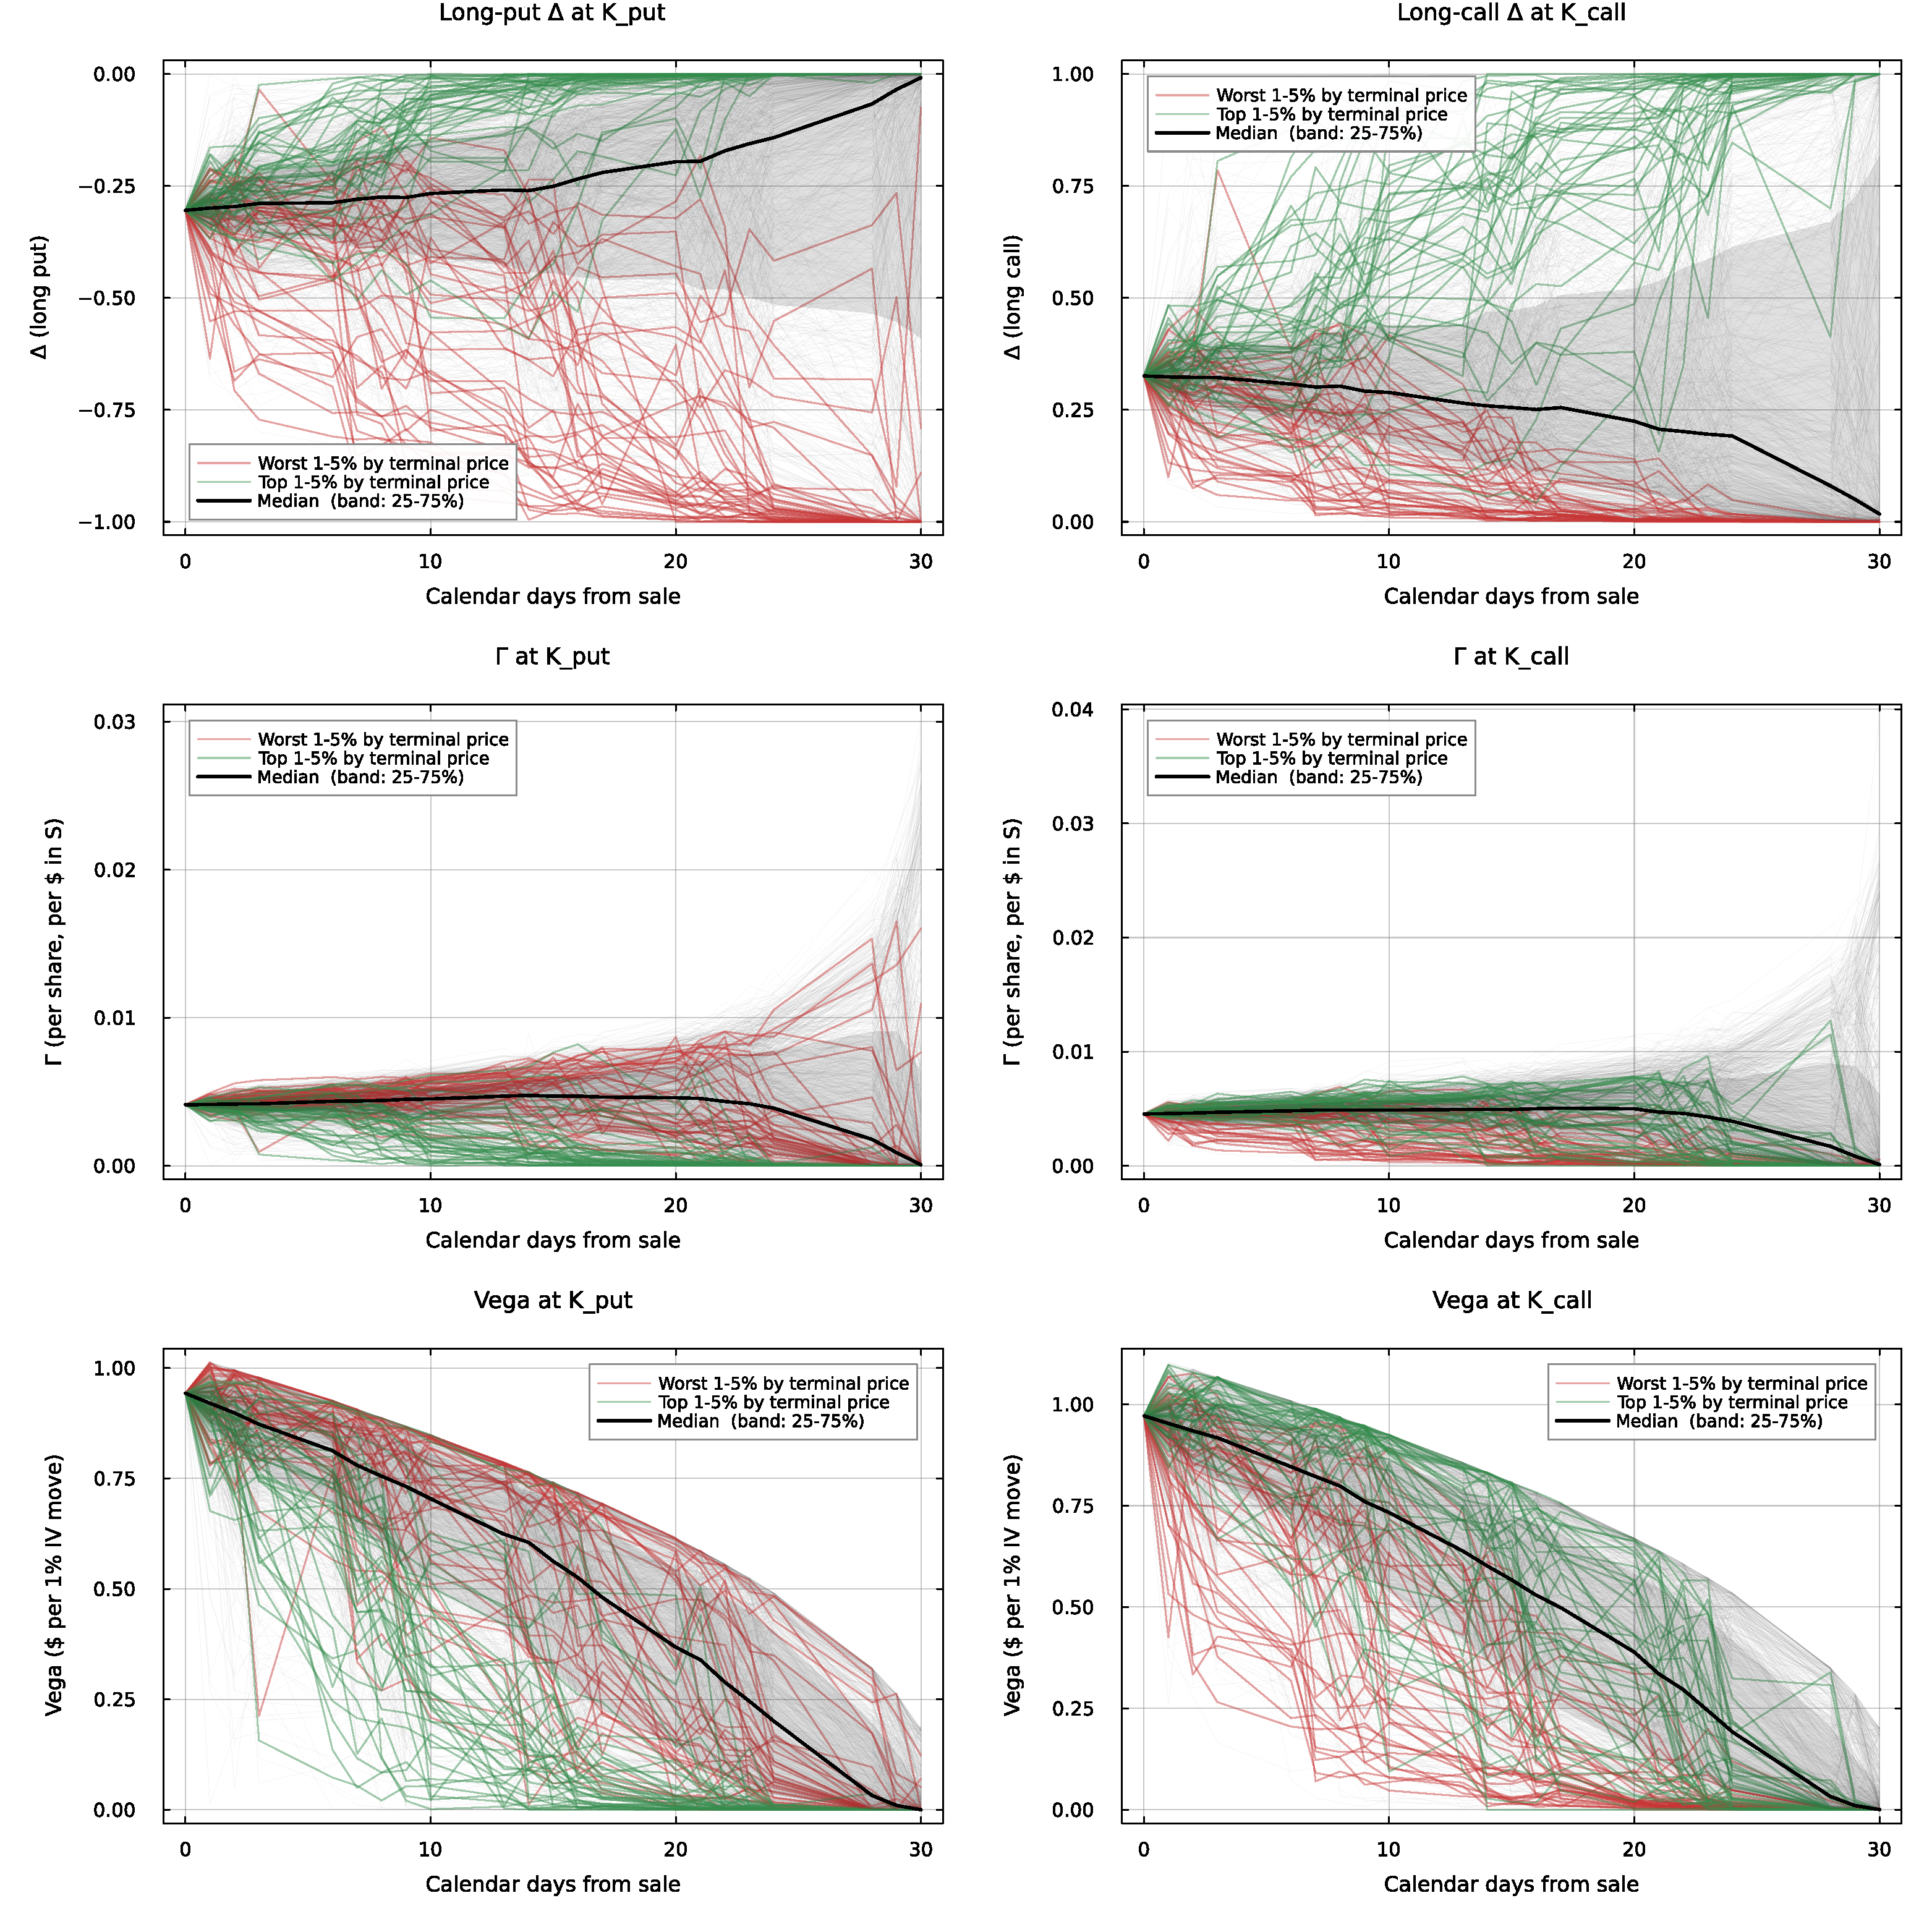
\includegraphics[width=\textwidth]{sections/figures/gs/gs_short_greeks.pdf}
\caption{Simulated evolution of GS long-option delta, gamma, and Vega along the stock paths. Sensitivities are calculated with the 201-step Leisen-Reimer pricer. Spot bumps were $1.5\%$ of spot, and IV bumps were 0.005. Vega is dollars per one volatility percentage point.}
\label{fig:gs_greeks}
\end{figure}

\FloatBarrier
\begin{table}[H]
\centering
\caption{Scenario results for LLY from 1{,}000 paths between April 28 and May 29, 2026. The horizon had 31 calendar days and 22 trading transitions. Dollar option values and P\&L are per share.}
\label{tab:lly_scenario}
\input{sections/generated/lly_scenario_table}
\end{table}

\FloatBarrier
\begin{figure}[H]
\centering

\includegraphics[width=\textwidth]{sections/figures/lly/lly_short_paths.pdf}
\caption{Simulated evolution of LLY stock prices (a), put values (b), and call values (c) along 1{,}000 paths between April 28 and May 29, 2026. The fitted surfaces included observations from this scenario period; these are illustrative paths, not an out-of-sample forecast. Time is measured in calendar days from April 28. Black curves show pointwise medians, and shading contains the middle 90\% of values. Red and blue curves show group medians for the 1st--5th and 95th--99th terminal-stock percentiles. Option values are dollars per share and represent repurchase costs for a short seller. Entry premiums were \$23.30 per share for the put and \$20.76 for the call.}
\label{fig:lly_paths}
\end{figure}

\begin{figure}[H]
\centering

\includegraphics[width=\textwidth]{sections/figures/lly/lly_iv_trajectories.pdf}
\caption{Simulated evolution of annualized IV at the LLY put strike (a) and call strike (b). Both panels express IV as percentages on the same vertical scale. Curves show pointwise medians across all 1{,}000 paths and within the terminal-stock groups in Supplementary Fig.~\ref{fig:lly_paths}; shading shows the 5th--95th percentile band. Time is measured in calendar days from April 28, 2026, and stops before expiration, when IV no longer enters the payoff.}
\label{fig:lly_iv}
\end{figure}

\begin{figure}[H]
\centering

\includegraphics[width=\textwidth]{sections/figures/lly/lly_short_greeks.pdf}
\caption{Simulated evolution of LLY long-option delta, gamma, and Vega along the stock paths. Sensitivities are calculated with the 201-step Leisen-Reimer pricer. Short-position Greeks have the opposite sign.}
\label{fig:lly_greeks}
\end{figure}
